\section{Origin of Mass: The Higgs Mechanism}\label{sec:higgs_mechanism}

    The derivation provided throughout the next three sections seeks to explain
        how the Higgs Mechanism is able to preserve the theory of gauge symmetry
        and largely follows the process laid out by Peskin\cite{Peskin_book}.
    To start, introduce a massless, scalar field $\phi$.
    The equation of motion for this field will be the Klein-Gordon equation
    \begin{equation} \begin{split}
        p^2 \phi = m^2 \phi
        \\(p^2 - m^2) \phi = 0
        \\(\partial^\mu \partial_\mu + m^2) \phi = 0
        \\\partial^\mu \partial_\mu \phi = 0,\; m\to0
        \quad.
    \end{split} \end{equation}

    By default, the Lagrangian for this field will be a trivial kinetic-only term
    \begin{equation}
        \Lag = K_{\phi} = \frac{1}{2} (\partial_{\mu} \phi)^2
        \quad.
    \end{equation}
    
    Next, introduce a quartic potential $U(\phi) = -\frac{1}{2} \mu^2 \phi^2 + \frac{\lambda}{4!} \phi^4$.
    Now the Lagrangian takes the form
    \begin{equation}
        \Lag = K_{\phi} - U_{\phi} = \frac{1}{2} (\partial_{\mu} \phi)^2 
            +\frac{1}{2} \mu^2 \phi^2 - \frac{\lambda}{4!} \phi^4
        \quad.
    \end{equation}
    Such a potential will result in a Hamiltonian which is symmetric about a local maximum at $\phi=0$.
    The Hamiltonian will have two minima to either side of $\phi=0$, at points $\pm v = \pm \sqrt{\frac{6}{\lambda}} \mu$.

    This is a small, seemingly innocuous change, so allow me to emphasize:
        this quartic potential is the linchpin of the entire Standard Model,
        and the origin of nearly all fundamental mass\footnote{
            Where ``fundamental mass'' refers to the mass of fundamental particles
                (except for that of neutrinos; the origin of neutrino mass is still a point of active research).
            Gluon binding energy is the actual source of most mass found in the baryonic matter of the universe
                (baryonic matter as opposed to \textit{dark matter},
                which is actually the vast majority of all mass in the universe
                and which is \textit{another} field of active research).
        } in the universe as it is currently understood.
    The reason for such a dramatic outcome begins with the fact that
        a system in such a potential will invariably fall into one of these minima.
    The Lagrangian can be rewritten from the perspective of one of these minima (e.g.\ $+v$),
        by substituting in a shifted field $h$, where $\phi(x)=v+h(x)$.
    \begin{equation} \begin{split} \label{eq:basic_higgs}
        \Lag & = \frac{1}{2} (\partial_{\mu} h)^2
            - \mu^2 h^2
            -\sqrt{\frac{\lambda}{6}} \mu h^3
            - \frac{\lambda}{4!} h^4 \\
         & = \frac{1}{2} (\partial_{\mu} h)^2
            - m^2_{h} h^2
            -\sqrt{\frac{\lambda}{6}} \mu h^3
            - \frac{\lambda}{4!} h^4 \\
        \quad.
    \end{split} \end{equation} %FIXME: you screwed up the terms somewhere

    \begin{figure}[h!]
        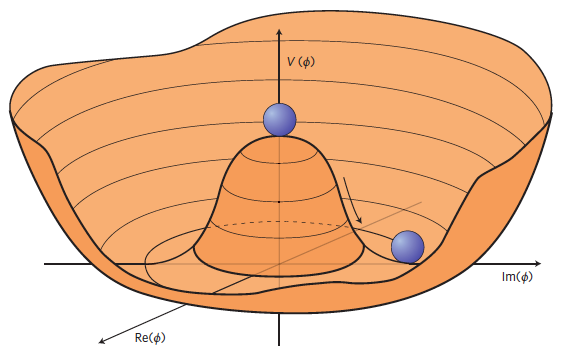
\includegraphics[width=\linewidth,height=\textheight,keepaspectratio]{theory/higgspotential}
        \caption{A two-dimensional representation of the Higgs Potential for a complex Higgs field.
            \cite{higgspotential}}
        \label{fig:higgs_potential}
    \end{figure}


    With the latter equation taking the form of a now massive field $h$ with both a three and four point self-coupling vertex.
    This is the mechanism used to take a massless, symmetric field and convert it to a massive, asymmetric form.
    In the next section, I will show how the same scalar field can induce mass in fields other than itself.


\section{Breaking Symmetry: GWS Theory}

    Based on the theory formulated by Glashow, Weinberg, and Salam (GWS Theory),
        I will now give the scalar field a complex phase and spinor components:
    \begin{equation}
        \vec{\phi}(x) = \frac{1}{\sqrt{2}} \tinymatrix{\phi_1 \\ \phi_2}
        \quad.
    \end{equation}
    $\vec{\phi}$ is still a scalar in space-time, but now also has vector components in the $SU(2)$ subspace.

    As with the Dirac fields, I will then impose $U(1) \times SU(2)$ gauge symmetry on the field, so it transforms as
    \begin{equation}
        \vec{\phi}(x) \rightarrow e^{i \alpha^a \tau^a} e^{i \beta/2 } \vec{\phi}(x)
        \quad.
    \end{equation}

    The additional symmetries will in general complicate matters significantly,
        but they do allow for one simplification which I will immediately utilize.
    Regardless of symmetries, any arbitrary vector such as $\vec{\phi}$ can be written as a unitary transformation $U(x)$ operating on a simpler single-valued vector
    \begin{equation}
        \vec{\phi}(x) = \frac{1}{\sqrt{2}} \tinymatrix{\phi_1 \\ \phi_2} = \frac{1}{\sqrt{2}} U(x) \tinymatrix{0 \\ \phi}
        \quad.
    \end{equation}
    Courtesy of the newly added gauge freedom, this field can be rotated through $SU(2) \times U(1)$ space freely without affecting the Lagrangian.
    A particularly convenient rotation to perform then, is one in alignment with the orientation of $U(x)$, such that $U(x)$ vanishes
    \begin{equation} \begin{split}
        \vec{\phi}(x) \rightarrow \vec{\phi}'(x) 
            &= U^{-1}(x) \vec{\phi}(x)
            = \frac{1}{\sqrt{2}} U^{-1}(x) U(x) \tinymatrix{0 \\ \phi}
            = \frac{1}{\sqrt{2}} \tinymatrix{0 \\ \phi} \\
        \vec{\phi}'(x) &= \frac{1}{\sqrt{2}} \tinymatrix{0 \\ \phi}
        \quad.
    \end{split} \end{equation}
    This orientation is referred as the \textit{Unitary Gauge}, and will be used for the rest of the chapter.

    Now for the complications.
    The added symmetries require that the derivative be changed to a covariant derivative 
        $D_{\mu} = \partial_{\mu} - \frac{ig}{2} \wField^a_{\mu} \sigma^a - \frac{ig'}{2} B_{\mu}$.
    Here, $\wField^a_\mu$ and $B_\mu$ correspond to the unbroken $SU(2)$ and $U(1)$ gauge fields respectively.
    This produces a Lagrangian:
    \begin{equation} \begin{split}
        \Lag &= \frac{1}{2} |D_{\mu} \vec{\phi}|^2 +
            \mu^2 \vec{\phi}^\dag \vec{\phi} - \lambda \left( \vec{\phi}^\dag\vec{\phi} \right)^2
        \quad.
    \end{split} \end{equation}


    Once again, I allow the scalar field to fall into its offset minimum $v$
        (hereafter refered to as the ``Vacuum Expectation Value'' or \textit{vev})
    \begin{equation}
        v \equiv \frac{\mu}{\sqrt{\lambda}} \textrm{ , for } \phi(x) \to h(x) + v
        \quad.
    \end{equation}
    Worth mentioning is that due to the added groups, there are no longer only two minima.
    Instead, there is now a continuum of equal-valued minima centered on a spherical ``valley'' a distance $v$ from $\phi=0$.
    Substituting into the Lagrangian now produces a more complex expression:
    \begin{equation} \begin{split}
        \label{eq:fullHiggs}
        \Lag & = \frac{1}{2} \left|D_{\mu} \minimatrix{0\\h(x)+v}\right|^2
            + \mu^2 \left|\minimatrix{0\\h(x)+v}\right|^2
            - \lambda \left|\minimatrix{0\\h(x)+v}\right|^4 \\
         & = \Lag_h + \Lag_v
        \quad.
    \end{split} \end{equation}
    where $\Lag_h$ takes a form similar to Eqn. \ref{eq:basic_higgs}, incorporating both the $h$ and $h$/$v$ cross terms.
    Meanwhile, $\Lag_v$ refers only to the terms arising from $D_{\mu}$ acting on the vev:
    \begin{equation}
        \label{eq:lagv}
        \Lag_v = \frac{1}{2} (D_{\mu} \vec{v})^2
        \quad.
    \end{equation}

    The expansion of this term specifically will lead to the breakdown of Electro-Weak Symmetry,
        and the $W$ and $Z$ bosons acquiring mass.

    %Get covariant derivative, evaluate at vev, pull out W,Z, and photon fields, and their masses (pg 722);
    Expanding only $D_{\mu} \vec{v}$ initially, the $\partial_{\mu}$ immediately vanishes ($v$ is a constant), yielding 
    \begin{equation} \begin{split}
        D^{\mu} v  = \big( \partial^{\mu} & - \frac{ig}{2} \wField^a_{\mu} \sigma^a - \frac{ig'}{2} B_{\mu} \big) \frac{1}{\sqrt{2}}\minimatrix{0\\v} \\
        = \big( & - \frac{ig}{2} \wField^a_{\mu} \sigma^a - \frac{ig'}{2} B_{\mu} \big) \frac{1}{\sqrt{2}}\minimatrix{0\\v} \\
        = - \frac{i}{2} \big( & g \wField^a_{\mu} \sigma^a + g' B_{\mu} \big) \frac{1}{\sqrt{2}}\minimatrix{0\\1} v
        \quad.
    \end{split} \end{equation}

    It is useful here to fully expand the $U(1) \times SU(2)$ fields into their matrix components and add them explicitly,
        as doing so reveals the origin of the photon and W and Z bosons.
    \begin{equation} \begin{split}
        g \wField^a_{\mu} \sigma^a + g' B_{\mu} & =
            g \wField^1_{\mu} \sigma^1
            + g \wField^2_{\mu} \sigma^2
            + g \wField^3_{\mu} \sigma^3
            + g' B_{\mu} I \\
        & = \begin{pmatrix}
            0 & g\wField^1_{\mu} \\ g\wField^1_{\mu} & 0 \end{pmatrix}
            + \begin{pmatrix} 0 & -ig\wField^2_{\mu} \\ ig\wField^2_{\mu} & 0 \end{pmatrix}
            + \begin{pmatrix} g\wField^3_{\mu} & 0 \\ 0 & -g\wField^3_{\mu} \end{pmatrix}
            + \begin{pmatrix} g'B_{\mu} & 0 \\ 0 & g'B_{\mu}
        \end{pmatrix} \\
        & = \begin{pmatrix} 
            g\wField^3_{\mu} + g'B_{\mu} & g\wField^1_{\mu} - ig\wField^2_{\mu} \\
            g\wField^1_{\mu} + ig\wField^2_{\mu} & -g\wField^3_{\mu} + g'B_{\mu}
        \end{pmatrix}
        \quad.
    \end{split} \end{equation}

    The four components of this matrix will ultimately be associated with the 
        gauge boson fields of the electromagnetic ($A$) and weak ($W$ \& $Z$) interactions
    \begin{equation} \begin{split}
        \label{eq:electroweak_matrix}
        \begin{pmatrix} 
            g\wField^3_{\mu} + g'B_{\mu} & g\wField^1_{\mu} - ig\wField^2_{\mu} \\
            g\wField^1_{\mu} + ig\wField^2_{\mu} & -g\wField^3_{\mu} + g'B_{\mu}
        \end{pmatrix} =
        \begin{pmatrix} 
            \sqrt{g^2 + g^{\prime 2}}\ A_{\mu} & g \sqrt{2}\ W^+_{\mu} \\
            g \sqrt{2}\ W^-_{\mu} & - \sqrt{g^2 + g^{\prime 2}}\ Z^0_{\mu}
        \end{pmatrix}
        \quad.
    \end{split} \end{equation}

    With $A$, $W^+$, $W^-$, and $Z^0$ related to the unbroken $\wField^a$ and $B$ fields by
    \begin{equation} \begin{split}
        A_{\mu} & = \frac{1}{\sqrt{g^2 + g^{\prime 2}}} ( g\wField^3_{\mu} + g'B_{\mu} ) \\
        Z^0_{\mu} & = \frac{1}{\sqrt{g^2 + g^{\prime 2}}} ( g\wField^3_{\mu} - g'B_{\mu} ) \\
        W^{\pm}_{\mu} & = \frac{1}{\sqrt{2}} (\wField^1_{\mu} \mp i\wField^2_{\mu})
        \quad.
    \end{split} \end{equation}

    The $\sqrt{g^2 + g^{\prime 2}}$ factor is the result of converting between
        $\tinymatrix{Z^0 \\ A}$ and $\tinymatrix{\wField^3 \\ B}$ by way of a rotation matrix
    \begin{equation} \begin{split}
        \begin{pmatrix} Z^0 \\ A \end{pmatrix} =
        \begin{pmatrix}
            \frac{g}{\sqrt{g^2 + g^{\prime 2}}} & \frac{-g'}{\sqrt{g^2 + g^{\prime 2}}} \\
            \frac{g'}{\sqrt{g^2 + g^{\prime 2}}} & \frac{g}{\sqrt{g^2 + g^{\prime 2}}}
        \end{pmatrix} \begin{pmatrix} \wField^3 \\ B \end{pmatrix} = 
        \begin{pmatrix}
            \cos\theta_w & -\sin\theta_w \\
            \sin\theta_w & \cos\theta_w
        \end{pmatrix} \begin{pmatrix} \wField^3 \\ B \end{pmatrix}
        \quad.
    \end{split} \end{equation}

    Where $\theta_w \equiv \cot(\frac{g'}{g})$ is known as the \textit{weak mixing angle} (AKA the Weinberg angle).

    Returning finally to Eqn. \ref{eq:lagv}, I now have
    \begin{equation} \begin{split}
        \label{eq:lagv_full}
        \Lag_v & = \frac{1}{2} (D_{\mu}^{ij} v_j)^2 \\
        & = \frac{1}{2}
            \frac{1}{\sqrt{2}} \begin{pmatrix} 0 & v \end{pmatrix}
            \left| -\frac{i}{2}
                \begin{pmatrix} 
                    \sqrt{g^2 + g^{\prime 2}}\ A_{\mu} & g \sqrt{2}\ W^+_{\mu} \\
                    g \sqrt{2}\ W^-_{\mu} & - \sqrt{g^2 + g^{\prime 2}}\ Z^0_{\mu}
                \end{pmatrix}
            \right|^2
            \frac{1}{\sqrt{2}} \begin{pmatrix} 0 \\ v \end{pmatrix} \\
        & = \frac{1}{2} \frac{v^2}{2} \frac{1}{4}
            \begin{pmatrix} 0 & 1 \end{pmatrix}
            \begin{pmatrix} 
                \sqrt{g^2 + g^{\prime 2}}\ A_{\mu} & g \sqrt{2}\ W^+_{\mu} \\
                g \sqrt{2}\ W^-_{\mu} & - \sqrt{g^2 + g^{\prime 2}}\ Z^0_{\mu}
            \end{pmatrix}
            \begin{pmatrix} 
                \sqrt{g^2 + g^{\prime 2}}\ A_{\mu} & g \sqrt{2}\ W^+_{\mu} \\
                g \sqrt{2}\ W^-_{\mu} & - \sqrt{g^2 + g^{\prime 2}}\ Z^0_{\mu}
            \end{pmatrix}
            \begin{pmatrix} 0 \\ 1 \end{pmatrix} \\
        & = \frac{1}{2} \frac{v^2}{2} \frac{1}{4}
            \begin{pmatrix} 
                g \sqrt{2}\ W^-_{\mu} & - \sqrt{g^2 + g^{\prime 2}}\ Z^0_{\mu}
            \end{pmatrix}
            \begin{pmatrix} 
                 g \sqrt{2}\ W^+_{\mu} \\
                 - \sqrt{g^2 + g^{\prime 2}}\ Z^0_{\mu}
            \end{pmatrix} \\
        & = \frac{1}{2} \frac{v^2}{2} \frac{1}{4} 
            \left[ 2 g^2  W^-_{\mu} W^+_{\mu}
            + \left(\sqrt{g^2 + g^{\prime 2}}\right)^2 (Z^0_{\mu})^2 \right] \\
        & = \frac{1}{2} \left[ \left(\frac{vg}{2}\right)^2\  W^-_{\mu} W^+_{\mu}
            + \frac{1}{2} \left(\frac{v}{2}\sqrt{g^2 + g^{\prime 2}}\right)\ (Z^0_{\mu})^2 \right] \\
        & = \frac{1}{2} \left[ m_W W^{-\ \mu} W^+_{\mu} + \frac{m_Z}{2} (Z^0_{\mu})^2 \right]
        \quad.
    \end{split} \end{equation}

    As in Section \ref{sec:higgs_mechanism}, the $W$ and $Z$ fields now have additional mass terms associated with their kinetic energy terms,
        with $m_W = \frac{vg}{2}$ and $m_Z = \left(\frac{v}{2}\sqrt{g^2 + g^{\prime 2}}\right) $.
    The photon field $A_{\mu}$ is notably absent in the final Lagrangian, and thus remains massless.
    A similar procedure can then be followed to allow the Higgs Field to interact with fermions
        (albeit with complications arising from mass-mixing and chirality),
        which will grant mass to the Dirac fields.


    % Fermion time!!
%\subsection{Giving Mass to Fermions}
% Ok this is seriously just the same thing but now we have to split the fermion fields into left and right and up-type and down-type
% and split the higgs into the higgs and conjugate higgs and also insert the complex mass matrix except don't insert it for charged leptons
% because reasons or something. And then poof your charged leptons have mass and your quarks have mass and flavour changing

    %Split fermions between right and left fields, assign LH to SU(2) doublets (T=+-1?), RH to SU(2) singlet (T=0), assign Y too (pg724-725);
    %Sandwitch covariant derivative terms between fermion fields, expand to get field currents (pg 725-726);
    %*Try* to expand masses and fail because of representation incompatibilities (pg 725);
    %Anamoly cancellation thing I'll probably ignore (pg 726);
    %Add higgs interaction psibar phi psi to fermion lagrangian, expand into higgs interaction, convert to fermion mass (pg 734);

%Further work must then be done to couple the higgs boson to fermions and itself
%You need to tie k2v, kl, and kv in to the shape of the higgs potential here
\section{Keystone of the Standard Model: The Higgs Boson} \label{sec:higgs_boson}

    With the critical role of the Higgs Field established, it is now time to return to Eqn. \ref{eq:fullHiggs},
        and investigate $\Lag_h$, the Lagrangian of the Higgs Boson itself.
    The terms involved therein provide information not only about the Higgs Field,
        but also provide insight into how the Higgs may be further studied:
    \begin{equation} \begin{split}
        \Lag &= \frac{1}{2} |D_{\mu} \vec{\phi}|^2 +
            \mu^2 \vec{\phi}^\dag \vec{\phi} - \lambda \left( \vec{\phi}^\dag\vec{\phi} \right)^2
        \\&= \Lag_K + \Lag_U
        \quad.
    \end{split} \end{equation}
    
    To make expansion easier, I will expand the covariant derivative terms ($\Lag_D$) first,
        and then add then expanded $\Lag_U$ terms.
    Starting with $\Lag_D$, (and defining $Q_{\mu}$ as the matrix from Eqn. \ref{eq:electroweak_matrix})

    \begin{equation} \begin{split}
        \Lag_D &= \frac{1}{2} |D_{\mu} \vec{\phi}|^2
            \\&= \frac{1}{2} (D^{\mu} \vec{\phi})^\dag (D_{\mu} \vec{\phi})
                = \frac{1}{2} \left[(\partial^{\mu} - \frac{i}{2}Q^{\mu}) \vec{\phi}\right]^\dag
                \left[(\partial_{\mu} - \frac{i}{2}Q^{\mu}) \vec{\phi}\right]
            \\&= \frac{1}{2} \left(\vec{\phi}^\dag \partial^{\mu} + \frac{i}{2} \vec{\phi}^\dag Q^{\mu \dag} \right)
                \left(\partial_{\mu}\vec{\phi} - \frac{i}{2}Q_{\mu}\vec{\phi} \right)
            \\&= \frac{1}{2} \left(
                \vec{\phi}^\dag \partial^{\mu} \partial_{\mu}\vec{\phi}
                - \frac{i}{2} \vec{\phi}^\dag \partial^{\mu} Q_{\mu}\vec{\phi}
                + \frac{i}{2} \vec{\phi}^\dag Q^{\mu \dag} \partial_{\mu}\vec{\phi}
                + \frac{1}{4} \vec{\phi}^\dag Q^{\mu \dag} Q_{\mu}\vec{\phi}
                \right)
            \\&= \frac{1}{2} \left(
                | \partial_{\mu}\vec{\phi} |^2
                + \frac{1}{4} \vec{\phi}^\dag Q^{\mu} Q_{\mu} \vec{\phi}
                \right)
                = \frac{1}{2} | \partial_{\mu}h |^2 + \frac{1}{8} \vec{\phi}^\dag Q^{\mu}Q_{\mu} \vec{\phi}
            \\&= \frac{1}{2} | \partial_{\mu}\vec{\phi} |^2 + \frac{1}{8} 
                    \minimatrix{0 & h^* + v} Q^{\mu}
                    Q_{\mu} \minimatrix{0 \\ h + v}
            \\&= \frac{1}{2} | \partial_{\mu}h |^2
                + \frac{1}{2} \left[ \left(\frac{g}{2}\right)^2\  W^{-\ \mu} W^+_{\mu}
                + \frac{1}{2} \left(\frac{1}{2}\sqrt{g^2 + g^{\prime 2}}\right)\ (Z^0_{\mu})^2 \right] (h+v)^2
        \quad.
    \end{split} \end{equation}

    The $(h+v)^2$ term will produce couplings quadratic in $v$ ($\Lag_v$ of Eqn. \ref{eq:lagv_full}), and both linear and quadratic in $h$.
    Replacing the coefficients in front of the $W$ and $Z$ fields with their respective masses

    \begin{equation} \begin{split}
        \Lag_D = \frac{1}{2} | \partial_{\mu}h |^2 + \Lag_v
            + 2v\left[ m_W W^{-\ \mu} W^+_{\mu} + \frac{m_Z}{2} (Z^0_{\mu})^2 \right] h
            + \left[ m_W W^{-\ \mu} W^+_{\mu} + \frac{m_Z}{2} (Z^0_{\mu})^2 \right] h^2
        \quad.
    \end{split} \end{equation}

    Often, $W$ and $Z$ field interactions are considered for the same process,
        and as such are described together simply as Vector Bosons, $V$:

    \begin{equation} \begin{split}
        \Lag_D = \frac{1}{2} | \partial_{\mu}h |^2 + \Lag_v
            + 2 v m_V V^2 h + m_V V^2 h^2
        \quad.
    \end{split} \end{equation}

    Returning to $\Lag_U$ and substituting in for $v$
    \begin{equation} \begin{split}
        \Lag_U &= \mu^2 \vec{\phi}^\dag \vec{\phi} - \lambda \left( \vec{\phi}^\dag\vec{\phi} \right)^2
        \\&= - \mu^2 h^2 -\lambda v h^3 - \frac{1}{4} \lambda h^4
        \\&= - \mu^2 h^2 - \mu \sqrt\lambda h^3 - \frac{1}{4} \lambda h^4
        \quad.
    \end{split} \end{equation}

    Identifying the Higgs mass $m_h$ as $\sqrt{2}\mu$,
        and the vev $v$ as $\frac{\mu}{\sqrt{\lambda}} = \frac{m_h}{\sqrt{2 \lambda}}$,
        I can now write the full Lagrangian for the Higgs field\cite{Halzen_book}
    \begin{equation} \begin{split} \label{eq:higgsfull}
        \Lag_h &= \Lag_D + \Lag_U
        \\&= \left[ \frac{1}{2} | \partial_{\mu}h |^2
            + m_h \sqrt{\frac{2}{\lambda}}  m_V V^2 h + m_V V^2 h^2 \right]
            + \left[ - \frac{1}{2} m^2_h h^2 - m_h \sqrt{\frac{\lambda}{2}} h^3 - \frac{1}{4} \lambda h^4 \right]
        \\&= \frac{1}{2} \left(\partial^2 - m_h^2 \right) h^2
            + m_h m_V \sqrt{\frac{2}{\lambda}} V^2 h + m_V V^2 h^2
            - m_h \sqrt{\frac{\lambda}{2}} h^3 - \frac{1}{4} \lambda h^4
        \quad.
    \end{split} \end{equation}

    The first term of this Lagrangian is simply the kinetic energy term for the Higgs.
    The remaining terms correspond, respectively,
        to the Higgs/Vector boson interaction,
        Higgs/Vector boson four-point interaction,
        Higgs self-coupling,
        and finally the Higgs four-point self-coupling.

    In 2012, the Higgs Boson was detected with a mass of 125 GeV, solidifying both its existence and crucial role in the Standard Model.
    More to the point, its detection confirmed the existence of the Higgs kinetic energy term in the Lagrangian,
        along with its coupling terms to fermions and vector bosons.
    The various self-interaction terms however, are still on more tenuous grounds.
    If they exist at all, there is no guarantee that these interactions have the coupling strength indicated by Eqn. \ref{eq:higgsfull}.
    In order to account for this uncertainty, the Lagrangian can be rewritten with arbitrary couplings for the interactions
    \begin{equation} \begin{split} \label{eq:higgskappas}
        \Lag_h &= \frac{1}{2} \left(\partial^2 - m_h^2 \right) h^2
            + \kv g_V V^2 h + \kvv g_{2V} V^2 h^2
            + \kl g_{\lambda} h^3 + \kappa_{2 \lambda} g_{\lambda} h^4
        \quad.
    \end{split} \end{equation}

    The new $\kappa$ terms are ratios of the coupling, as predicted by the Standard Model ($g$), to the true coupling value ($g'$).
    For example, $\kappa_V \equiv \frac{g'_V}{g_V} = \frac{g'_V}{m_h m_V \sqrt{2/\lambda}}$.
    A $\kappa$ value of 1 indicates consistency with the coupling strength predicted by the Standard Model.
    Any value other than 1 would indicate deviation from the Standard Model,
        which would need to be explained with a modification to the (or entirely new) theory.
    As of 2020, $\kv$ has been measured at a value of $1.05 \pm 0.04$,
        based on combined analysis of single Higgs production processes\cite{paper:higgs_combined}.
    The couplings $\kvv$, $\kl$, and $\kappa_{2\lambda}$ however, do not significantly affect the production of single Higgs processes.
    The quartic coupling $\kappa_{2\lambda}$ is outside the scope of this thesis,
        but $\kvv$ and $\kl$ can be measured through their effect on di-Higgs production.
    Constraining the range of these values could yield key insight into the validity of the Standard Model and the nature of the Higgs Potential,
        and will therefore be the target of this thesis.
